% Created by tikzDevice version 0.10.1 on 2018-02-07 13:30:58
% !TEX encoding = UTF-8 Unicode
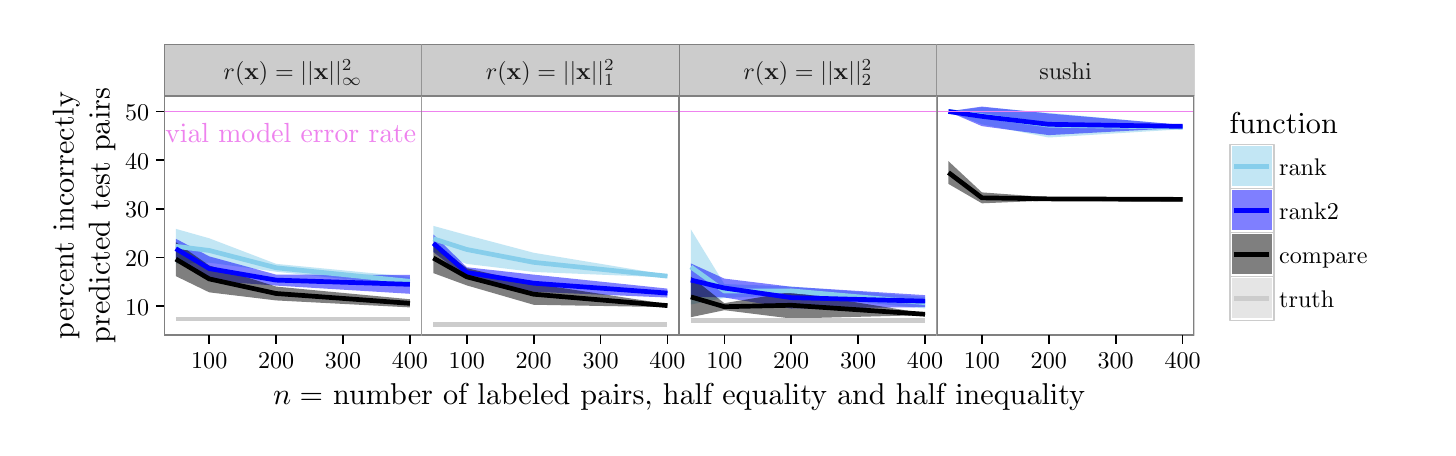
\begin{tikzpicture}[x=1pt,y=1pt]
\definecolor{fillColor}{RGB}{255,255,255}
\path[use as bounding box,fill=fillColor,fill opacity=0.00] (0,0) rectangle (505.89,144.54);
\begin{scope}
\path[clip] (  0.00,  0.00) rectangle (505.89,144.54);
\definecolor{drawColor}{RGB}{255,255,255}
\definecolor{fillColor}{RGB}{255,255,255}

\path[draw=drawColor,line width= 0.6pt,line join=round,line cap=round,fill=fillColor] ( -0.00, -0.00) rectangle (505.89,144.54);
\end{scope}
\begin{scope}
\path[clip] ( 49.29,119.96) rectangle (142.36,138.54);
\definecolor{drawColor}{gray}{0.50}
\definecolor{fillColor}{gray}{0.80}

\path[draw=drawColor,line width= 0.2pt,line join=round,line cap=round,fill=fillColor] ( 49.29,119.96) rectangle (142.36,138.54);
\definecolor{drawColor}{gray}{0.10}

\node[text=drawColor,anchor=base,inner sep=0pt, outer sep=0pt, scale=  0.87] at ( 95.82,125.96) {$r(\mathbf x) = ||\mathbf x||_\infty^2$};
\end{scope}
\begin{scope}
\path[clip] (142.36,119.96) rectangle (235.42,138.54);
\definecolor{drawColor}{gray}{0.50}
\definecolor{fillColor}{gray}{0.80}

\path[draw=drawColor,line width= 0.2pt,line join=round,line cap=round,fill=fillColor] (142.36,119.96) rectangle (235.42,138.54);
\definecolor{drawColor}{gray}{0.10}

\node[text=drawColor,anchor=base,inner sep=0pt, outer sep=0pt, scale=  0.87] at (188.89,125.96) {$r(\mathbf x) = ||\mathbf x||_1^2$};
\end{scope}
\begin{scope}
\path[clip] (235.42,119.96) rectangle (328.49,138.54);
\definecolor{drawColor}{gray}{0.50}
\definecolor{fillColor}{gray}{0.80}

\path[draw=drawColor,line width= 0.2pt,line join=round,line cap=round,fill=fillColor] (235.42,119.96) rectangle (328.49,138.54);
\definecolor{drawColor}{gray}{0.10}

\node[text=drawColor,anchor=base,inner sep=0pt, outer sep=0pt, scale=  0.87] at (281.96,125.96) {$r(\mathbf x) = ||\mathbf x||_2^2$};
\end{scope}
\begin{scope}
\path[clip] (328.49,119.96) rectangle (421.56,138.54);
\definecolor{drawColor}{gray}{0.50}
\definecolor{fillColor}{gray}{0.80}

\path[draw=drawColor,line width= 0.2pt,line join=round,line cap=round,fill=fillColor] (328.49,119.96) rectangle (421.56,138.54);
\definecolor{drawColor}{gray}{0.10}

\node[text=drawColor,anchor=base,inner sep=0pt, outer sep=0pt, scale=  0.87] at (375.02,125.96) {sushi};
\end{scope}
\begin{scope}
\path[clip] ( 49.29, 33.41) rectangle (142.36,119.96);
\definecolor{fillColor}{RGB}{255,255,255}

\path[fill=fillColor] ( 49.29, 33.41) rectangle (142.36,119.96);
\definecolor{fillColor}{RGB}{135,206,235}

\path[fill=fillColor,fill opacity=0.50] ( 53.52, 71.84) --
	( 65.61, 68.43) --
	( 89.78, 59.19) --
	(138.13, 54.51) --
	(138.13, 51.24) --
	( 89.78, 56.36) --
	( 65.61, 59.63) --
	( 53.52, 59.24) --
	cycle;
\definecolor{fillColor}{RGB}{0,0,255}

\path[fill=fillColor,fill opacity=0.50] ( 53.52, 68.26) --
	( 65.61, 61.90) --
	( 89.78, 55.30) --
	(138.13, 55.20) --
	(138.13, 48.38) --
	( 89.78, 51.34) --
	( 65.61, 53.08) --
	( 53.52, 61.13) --
	cycle;
\definecolor{fillColor}{RGB}{0,0,0}

\path[fill=fillColor,fill opacity=0.50] ( 53.52, 67.04) --
	( 65.61, 58.59) --
	( 89.78, 50.98) --
	(138.13, 46.40) --
	(138.13, 43.46) --
	( 89.78, 45.98) --
	( 65.61, 48.90) --
	( 53.52, 54.77) --
	cycle;
\definecolor{fillColor}{RGB}{204,204,204}

\path[fill=fillColor,fill opacity=0.50] ( 53.52, 39.31) --
	( 65.61, 39.31) --
	( 89.78, 39.31) --
	(138.13, 39.31) --
	(138.13, 39.31) --
	( 89.78, 39.31) --
	( 65.61, 39.31) --
	( 53.52, 39.31) --
	cycle;
\definecolor{drawColor}{RGB}{135,206,235}

\path[draw=drawColor,line width= 1.7pt,line join=round] ( 53.52, 65.54) --
	( 65.61, 64.03) --
	( 89.78, 57.78) --
	(138.13, 52.87);
\definecolor{drawColor}{RGB}{0,0,255}

\path[draw=drawColor,line width= 1.7pt,line join=round] ( 53.52, 64.69) --
	( 65.61, 57.49) --
	( 89.78, 53.32) --
	(138.13, 51.79);
\definecolor{drawColor}{RGB}{0,0,0}

\path[draw=drawColor,line width= 1.7pt,line join=round] ( 53.52, 60.91) --
	( 65.61, 53.75) --
	( 89.78, 48.48) --
	(138.13, 44.93);
\definecolor{drawColor}{gray}{0.80}

\path[draw=drawColor,line width= 1.7pt,line join=round] ( 53.52, 39.31) --
	( 65.61, 39.31) --
	( 89.78, 39.31) --
	(138.13, 39.31);
\definecolor{drawColor}{RGB}{238,130,238}

\path[draw=drawColor,line width= 0.6pt,line join=round] ( 49.29,114.27) -- (142.36,114.27);

\node[text=drawColor,anchor=base,inner sep=0pt, outer sep=0pt, scale=  1.00] at ( 89.78,102.91) {trivial model error rate};
\definecolor{drawColor}{gray}{0.50}

\path[draw=drawColor,line width= 0.6pt,line join=round,line cap=round] ( 49.29, 33.41) rectangle (142.36,119.96);
\end{scope}
\begin{scope}
\path[clip] (142.36, 33.41) rectangle (235.42,119.96);
\definecolor{fillColor}{RGB}{255,255,255}

\path[fill=fillColor] (142.36, 33.41) rectangle (235.42,119.96);
\definecolor{fillColor}{RGB}{135,206,235}

\path[fill=fillColor,fill opacity=0.50] (146.59, 72.91) --
	(158.67, 69.59) --
	(182.85, 63.20) --
	(231.19, 55.20) --
	(231.19, 54.30) --
	(182.85, 56.27) --
	(158.67, 59.18) --
	(146.59, 63.63) --
	cycle;
\definecolor{fillColor}{RGB}{0,0,255}

\path[fill=fillColor,fill opacity=0.50] (146.59, 69.78) --
	(158.67, 57.97) --
	(182.85, 55.30) --
	(231.19, 50.25) --
	(231.19, 47.02) --
	(182.85, 49.11) --
	(158.67, 54.14) --
	(146.59, 63.45) --
	cycle;
\definecolor{fillColor}{RGB}{0,0,0}

\path[fill=fillColor,fill opacity=0.50] (146.59, 66.75) --
	(158.67, 57.62) --
	(182.85, 52.02) --
	(231.19, 44.67) --
	(231.19, 43.56) --
	(182.85, 44.41) --
	(158.67, 51.41) --
	(146.59, 55.85) --
	cycle;
\definecolor{fillColor}{RGB}{204,204,204}

\path[fill=fillColor,fill opacity=0.50] (146.59, 37.34) --
	(158.67, 37.34) --
	(182.85, 37.34) --
	(231.19, 37.34) --
	(231.19, 37.34) --
	(182.85, 37.34) --
	(158.67, 37.34) --
	(146.59, 37.34) --
	cycle;
\definecolor{drawColor}{RGB}{135,206,235}

\path[draw=drawColor,line width= 1.7pt,line join=round] (146.59, 68.27) --
	(158.67, 64.38) --
	(182.85, 59.74) --
	(231.19, 54.75);
\definecolor{drawColor}{RGB}{0,0,255}

\path[draw=drawColor,line width= 1.7pt,line join=round] (146.59, 66.62) --
	(158.67, 56.06) --
	(182.85, 52.20) --
	(231.19, 48.63);
\definecolor{drawColor}{RGB}{0,0,0}

\path[draw=drawColor,line width= 1.7pt,line join=round] (146.59, 61.30) --
	(158.67, 54.51) --
	(182.85, 48.22) --
	(231.19, 44.11);
\definecolor{drawColor}{gray}{0.80}

\path[draw=drawColor,line width= 1.7pt,line join=round] (146.59, 37.34) --
	(158.67, 37.34) --
	(182.85, 37.34) --
	(231.19, 37.34);
\definecolor{drawColor}{RGB}{238,130,238}

\path[draw=drawColor,line width= 0.6pt,line join=round] (142.36,114.27) -- (235.42,114.27);
\definecolor{drawColor}{gray}{0.50}

\path[draw=drawColor,line width= 0.6pt,line join=round,line cap=round] (142.36, 33.41) rectangle (235.42,119.96);
\end{scope}
\begin{scope}
\path[clip] (235.42, 33.41) rectangle (328.49,119.96);
\definecolor{fillColor}{RGB}{255,255,255}

\path[fill=fillColor] (235.42, 33.41) rectangle (328.49,119.96);
\definecolor{fillColor}{RGB}{135,206,235}

\path[fill=fillColor,fill opacity=0.50] (239.65, 71.63) --
	(251.74, 51.89) --
	(275.91, 51.03) --
	(324.26, 47.27) --
	(324.26, 43.08) --
	(275.91, 47.86) --
	(251.74, 46.87) --
	(239.65, 44.52) --
	cycle;
\definecolor{fillColor}{RGB}{0,0,255}

\path[fill=fillColor,fill opacity=0.50] (239.65, 59.34) --
	(251.74, 53.87) --
	(275.91, 50.92) --
	(324.26, 47.89) --
	(324.26, 43.55) --
	(275.91, 43.06) --
	(251.74, 47.05) --
	(239.65, 47.32) --
	cycle;
\definecolor{fillColor}{RGB}{0,0,0}

\path[fill=fillColor,fill opacity=0.50] (239.65, 54.58) --
	(251.74, 44.98) --
	(275.91, 49.02) --
	(324.26, 41.29) --
	(324.26, 40.67) --
	(275.91, 39.44) --
	(251.74, 42.45) --
	(239.65, 39.92) --
	cycle;
\definecolor{fillColor}{RGB}{204,204,204}

\path[fill=fillColor,fill opacity=0.50] (239.65, 38.75) --
	(251.74, 38.75) --
	(275.91, 38.75) --
	(324.26, 38.75) --
	(324.26, 38.75) --
	(275.91, 38.75) --
	(251.74, 38.75) --
	(239.65, 38.75) --
	cycle;
\definecolor{drawColor}{RGB}{135,206,235}

\path[draw=drawColor,line width= 1.7pt,line join=round] (239.65, 58.08) --
	(251.74, 49.38) --
	(275.91, 49.44) --
	(324.26, 45.17);
\definecolor{drawColor}{RGB}{0,0,255}

\path[draw=drawColor,line width= 1.7pt,line join=round] (239.65, 53.33) --
	(251.74, 50.46) --
	(275.91, 46.99) --
	(324.26, 45.72);
\definecolor{drawColor}{RGB}{0,0,0}

\path[draw=drawColor,line width= 1.7pt,line join=round] (239.65, 47.25) --
	(251.74, 43.71) --
	(275.91, 44.23) --
	(324.26, 40.98);
\definecolor{drawColor}{gray}{0.80}

\path[draw=drawColor,line width= 1.7pt,line join=round] (239.65, 38.75) --
	(251.74, 38.75) --
	(275.91, 38.75) --
	(324.26, 38.75);
\definecolor{drawColor}{RGB}{238,130,238}

\path[draw=drawColor,line width= 0.6pt,line join=round] (235.42,114.27) -- (328.49,114.27);
\definecolor{drawColor}{gray}{0.50}

\path[draw=drawColor,line width= 0.6pt,line join=round,line cap=round] (235.42, 33.41) rectangle (328.49,119.96);
\end{scope}
\begin{scope}
\path[clip] (328.49, 33.41) rectangle (421.56,119.96);
\definecolor{fillColor}{RGB}{255,255,255}

\path[fill=fillColor] (328.49, 33.41) rectangle (421.56,119.96);
\definecolor{fillColor}{RGB}{135,206,235}

\path[fill=fillColor,fill opacity=0.50] (332.72,114.27) --
	(344.81,115.82) --
	(368.98,113.76) --
	(417.33,109.31) --
	(417.33,107.84) --
	(368.98,104.85) --
	(344.81,109.61) --
	(332.72,114.27) --
	cycle;
\definecolor{fillColor}{RGB}{0,0,255}

\path[fill=fillColor,fill opacity=0.50] (332.72,114.29) --
	(344.81,116.02) --
	(368.98,113.52) --
	(417.33,109.40) --
	(417.33,108.35) --
	(368.98,105.71) --
	(344.81,108.96) --
	(332.72,114.20) --
	cycle;
\definecolor{fillColor}{RGB}{0,0,0}

\path[fill=fillColor,fill opacity=0.50] (332.72, 96.29) --
	(344.81, 85.02) --
	(368.98, 83.26) --
	(417.33, 83.31) --
	(417.33, 81.66) --
	(368.98, 82.07) --
	(344.81, 81.07) --
	(332.72, 88.08) --
	cycle;
\definecolor{drawColor}{RGB}{135,206,235}

\path[draw=drawColor,line width= 1.7pt,line join=round] (332.72,114.27) --
	(344.81,112.72) --
	(368.98,109.30) --
	(417.33,108.57);
\definecolor{drawColor}{RGB}{0,0,255}

\path[draw=drawColor,line width= 1.7pt,line join=round] (332.72,114.25) --
	(344.81,112.49) --
	(368.98,109.62) --
	(417.33,108.88);
\definecolor{drawColor}{RGB}{0,0,0}

\path[draw=drawColor,line width= 1.7pt,line join=round] (332.72, 92.18) --
	(344.81, 83.05) --
	(368.98, 82.67) --
	(417.33, 82.49);
\definecolor{drawColor}{RGB}{238,130,238}

\path[draw=drawColor,line width= 0.6pt,line join=round] (328.49,114.27) -- (421.56,114.27);
\definecolor{drawColor}{gray}{0.50}

\path[draw=drawColor,line width= 0.6pt,line join=round,line cap=round] (328.49, 33.41) rectangle (421.56,119.96);
\end{scope}
\begin{scope}
\path[clip] (  0.00,  0.00) rectangle (505.89,144.54);
\definecolor{drawColor}{RGB}{0,0,0}

\node[text=drawColor,anchor=base east,inner sep=0pt, outer sep=0pt, scale=  0.87] at ( 43.89, 40.58) {10};

\node[text=drawColor,anchor=base east,inner sep=0pt, outer sep=0pt, scale=  0.87] at ( 43.89, 58.18) {20};

\node[text=drawColor,anchor=base east,inner sep=0pt, outer sep=0pt, scale=  0.87] at ( 43.89, 75.78) {30};

\node[text=drawColor,anchor=base east,inner sep=0pt, outer sep=0pt, scale=  0.87] at ( 43.89, 93.38) {40};

\node[text=drawColor,anchor=base east,inner sep=0pt, outer sep=0pt, scale=  0.87] at ( 43.89,110.98) {50};
\end{scope}
\begin{scope}
\path[clip] (  0.00,  0.00) rectangle (505.89,144.54);
\definecolor{drawColor}{RGB}{0,0,0}

\path[draw=drawColor,line width= 0.6pt,line join=round] ( 46.29, 43.87) --
	( 49.29, 43.87);

\path[draw=drawColor,line width= 0.6pt,line join=round] ( 46.29, 61.47) --
	( 49.29, 61.47);

\path[draw=drawColor,line width= 0.6pt,line join=round] ( 46.29, 79.07) --
	( 49.29, 79.07);

\path[draw=drawColor,line width= 0.6pt,line join=round] ( 46.29, 96.67) --
	( 49.29, 96.67);

\path[draw=drawColor,line width= 0.6pt,line join=round] ( 46.29,114.27) --
	( 49.29,114.27);
\end{scope}
\begin{scope}
\path[clip] (  0.00,  0.00) rectangle (505.89,144.54);
\definecolor{drawColor}{RGB}{0,0,0}

\path[draw=drawColor,line width= 0.6pt,line join=round] ( 65.61, 30.41) --
	( 65.61, 33.41);

\path[draw=drawColor,line width= 0.6pt,line join=round] ( 89.78, 30.41) --
	( 89.78, 33.41);

\path[draw=drawColor,line width= 0.6pt,line join=round] (113.95, 30.41) --
	(113.95, 33.41);

\path[draw=drawColor,line width= 0.6pt,line join=round] (138.13, 30.41) --
	(138.13, 33.41);
\end{scope}
\begin{scope}
\path[clip] (  0.00,  0.00) rectangle (505.89,144.54);
\definecolor{drawColor}{RGB}{0,0,0}

\node[text=drawColor,anchor=base,inner sep=0pt, outer sep=0pt, scale=  0.87] at ( 65.61, 21.43) {100};

\node[text=drawColor,anchor=base,inner sep=0pt, outer sep=0pt, scale=  0.87] at ( 89.78, 21.43) {200};

\node[text=drawColor,anchor=base,inner sep=0pt, outer sep=0pt, scale=  0.87] at (113.95, 21.43) {300};

\node[text=drawColor,anchor=base,inner sep=0pt, outer sep=0pt, scale=  0.87] at (138.13, 21.43) {400};
\end{scope}
\begin{scope}
\path[clip] (  0.00,  0.00) rectangle (505.89,144.54);
\definecolor{drawColor}{RGB}{0,0,0}

\path[draw=drawColor,line width= 0.6pt,line join=round] (158.67, 30.41) --
	(158.67, 33.41);

\path[draw=drawColor,line width= 0.6pt,line join=round] (182.85, 30.41) --
	(182.85, 33.41);

\path[draw=drawColor,line width= 0.6pt,line join=round] (207.02, 30.41) --
	(207.02, 33.41);

\path[draw=drawColor,line width= 0.6pt,line join=round] (231.19, 30.41) --
	(231.19, 33.41);
\end{scope}
\begin{scope}
\path[clip] (  0.00,  0.00) rectangle (505.89,144.54);
\definecolor{drawColor}{RGB}{0,0,0}

\node[text=drawColor,anchor=base,inner sep=0pt, outer sep=0pt, scale=  0.87] at (158.67, 21.43) {100};

\node[text=drawColor,anchor=base,inner sep=0pt, outer sep=0pt, scale=  0.87] at (182.85, 21.43) {200};

\node[text=drawColor,anchor=base,inner sep=0pt, outer sep=0pt, scale=  0.87] at (207.02, 21.43) {300};

\node[text=drawColor,anchor=base,inner sep=0pt, outer sep=0pt, scale=  0.87] at (231.19, 21.43) {400};
\end{scope}
\begin{scope}
\path[clip] (  0.00,  0.00) rectangle (505.89,144.54);
\definecolor{drawColor}{RGB}{0,0,0}

\path[draw=drawColor,line width= 0.6pt,line join=round] (251.74, 30.41) --
	(251.74, 33.41);

\path[draw=drawColor,line width= 0.6pt,line join=round] (275.91, 30.41) --
	(275.91, 33.41);

\path[draw=drawColor,line width= 0.6pt,line join=round] (300.09, 30.41) --
	(300.09, 33.41);

\path[draw=drawColor,line width= 0.6pt,line join=round] (324.26, 30.41) --
	(324.26, 33.41);
\end{scope}
\begin{scope}
\path[clip] (  0.00,  0.00) rectangle (505.89,144.54);
\definecolor{drawColor}{RGB}{0,0,0}

\node[text=drawColor,anchor=base,inner sep=0pt, outer sep=0pt, scale=  0.87] at (251.74, 21.43) {100};

\node[text=drawColor,anchor=base,inner sep=0pt, outer sep=0pt, scale=  0.87] at (275.91, 21.43) {200};

\node[text=drawColor,anchor=base,inner sep=0pt, outer sep=0pt, scale=  0.87] at (300.09, 21.43) {300};

\node[text=drawColor,anchor=base,inner sep=0pt, outer sep=0pt, scale=  0.87] at (324.26, 21.43) {400};
\end{scope}
\begin{scope}
\path[clip] (  0.00,  0.00) rectangle (505.89,144.54);
\definecolor{drawColor}{RGB}{0,0,0}

\path[draw=drawColor,line width= 0.6pt,line join=round] (344.81, 30.41) --
	(344.81, 33.41);

\path[draw=drawColor,line width= 0.6pt,line join=round] (368.98, 30.41) --
	(368.98, 33.41);

\path[draw=drawColor,line width= 0.6pt,line join=round] (393.15, 30.41) --
	(393.15, 33.41);

\path[draw=drawColor,line width= 0.6pt,line join=round] (417.33, 30.41) --
	(417.33, 33.41);
\end{scope}
\begin{scope}
\path[clip] (  0.00,  0.00) rectangle (505.89,144.54);
\definecolor{drawColor}{RGB}{0,0,0}

\node[text=drawColor,anchor=base,inner sep=0pt, outer sep=0pt, scale=  0.87] at (344.81, 21.43) {100};

\node[text=drawColor,anchor=base,inner sep=0pt, outer sep=0pt, scale=  0.87] at (368.98, 21.43) {200};

\node[text=drawColor,anchor=base,inner sep=0pt, outer sep=0pt, scale=  0.87] at (393.15, 21.43) {300};

\node[text=drawColor,anchor=base,inner sep=0pt, outer sep=0pt, scale=  0.87] at (417.33, 21.43) {400};
\end{scope}
\begin{scope}
\path[clip] (  0.00,  0.00) rectangle (505.89,144.54);
\definecolor{drawColor}{RGB}{0,0,0}

\node[text=drawColor,anchor=base,inner sep=0pt, outer sep=0pt, scale=  1.09] at (235.42,  8.40) {$n=$ number of labeled pairs, half equality and half inequality};
\end{scope}
\begin{scope}
\path[clip] (  0.00,  0.00) rectangle (505.89,144.54);
\definecolor{drawColor}{RGB}{0,0,0}

\node[text=drawColor,rotate= 90.00,anchor=base,inner sep=0pt, outer sep=0pt, scale=  1.09] at ( 16.63, 76.68) {percent incorrectly};

\node[text=drawColor,rotate= 90.00,anchor=base,inner sep=0pt, outer sep=0pt, scale=  1.09] at ( 29.59, 76.68) {predicted test pairs};
\end{scope}
\begin{scope}
\path[clip] (  0.00,  0.00) rectangle (505.89,144.54);
\definecolor{fillColor}{RGB}{255,255,255}

\path[fill=fillColor] (430.09, 34.52) rectangle (491.35,118.85);
\end{scope}
\begin{scope}
\path[clip] (  0.00,  0.00) rectangle (505.89,144.54);
\definecolor{drawColor}{RGB}{0,0,0}

\node[text=drawColor,anchor=base west,inner sep=0pt, outer sep=0pt, scale=  1.09] at (434.36,106.36) {function};
\end{scope}
\begin{scope}
\path[clip] (  0.00,  0.00) rectangle (505.89,144.54);
\definecolor{drawColor}{gray}{0.80}
\definecolor{fillColor}{RGB}{255,255,255}

\path[draw=drawColor,line width= 0.6pt,line join=round,line cap=round,fill=fillColor] (434.36, 86.48) rectangle (450.26,102.38);
\end{scope}
\begin{scope}
\path[clip] (  0.00,  0.00) rectangle (505.89,144.54);
\definecolor{fillColor}{RGB}{135,206,235}

\path[fill=fillColor,fill opacity=0.50] (435.07, 87.19) rectangle (449.55,101.67);
\end{scope}
\begin{scope}
\path[clip] (  0.00,  0.00) rectangle (505.89,144.54);
\definecolor{drawColor}{RGB}{135,206,235}

\path[draw=drawColor,line width= 1.7pt,line join=round] (435.95, 94.43) -- (448.67, 94.43);
\end{scope}
\begin{scope}
\path[clip] (  0.00,  0.00) rectangle (505.89,144.54);
\definecolor{drawColor}{gray}{0.80}
\definecolor{fillColor}{RGB}{255,255,255}

\path[draw=drawColor,line width= 0.6pt,line join=round,line cap=round,fill=fillColor] (434.36, 70.58) rectangle (450.26, 86.48);
\end{scope}
\begin{scope}
\path[clip] (  0.00,  0.00) rectangle (505.89,144.54);
\definecolor{fillColor}{RGB}{0,0,255}

\path[fill=fillColor,fill opacity=0.50] (435.07, 71.29) rectangle (449.55, 85.77);
\end{scope}
\begin{scope}
\path[clip] (  0.00,  0.00) rectangle (505.89,144.54);
\definecolor{drawColor}{RGB}{0,0,255}

\path[draw=drawColor,line width= 1.7pt,line join=round] (435.95, 78.53) -- (448.67, 78.53);
\end{scope}
\begin{scope}
\path[clip] (  0.00,  0.00) rectangle (505.89,144.54);
\definecolor{drawColor}{gray}{0.80}
\definecolor{fillColor}{RGB}{255,255,255}

\path[draw=drawColor,line width= 0.6pt,line join=round,line cap=round,fill=fillColor] (434.36, 54.68) rectangle (450.26, 70.58);
\end{scope}
\begin{scope}
\path[clip] (  0.00,  0.00) rectangle (505.89,144.54);
\definecolor{fillColor}{RGB}{0,0,0}

\path[fill=fillColor,fill opacity=0.50] (435.07, 55.39) rectangle (449.55, 69.87);
\end{scope}
\begin{scope}
\path[clip] (  0.00,  0.00) rectangle (505.89,144.54);
\definecolor{drawColor}{RGB}{0,0,0}

\path[draw=drawColor,line width= 1.7pt,line join=round] (435.95, 62.63) -- (448.67, 62.63);
\end{scope}
\begin{scope}
\path[clip] (  0.00,  0.00) rectangle (505.89,144.54);
\definecolor{drawColor}{gray}{0.80}
\definecolor{fillColor}{RGB}{255,255,255}

\path[draw=drawColor,line width= 0.6pt,line join=round,line cap=round,fill=fillColor] (434.36, 38.78) rectangle (450.26, 54.68);
\end{scope}
\begin{scope}
\path[clip] (  0.00,  0.00) rectangle (505.89,144.54);
\definecolor{fillColor}{RGB}{204,204,204}

\path[fill=fillColor,fill opacity=0.50] (435.07, 39.50) rectangle (449.55, 53.97);
\end{scope}
\begin{scope}
\path[clip] (  0.00,  0.00) rectangle (505.89,144.54);
\definecolor{drawColor}{gray}{0.80}

\path[draw=drawColor,line width= 1.7pt,line join=round] (435.95, 46.73) -- (448.67, 46.73);
\end{scope}
\begin{scope}
\path[clip] (  0.00,  0.00) rectangle (505.89,144.54);
\definecolor{drawColor}{RGB}{0,0,0}

\node[text=drawColor,anchor=base west,inner sep=0pt, outer sep=0pt, scale=  0.87] at (452.25, 91.14) {rank};
\end{scope}
\begin{scope}
\path[clip] (  0.00,  0.00) rectangle (505.89,144.54);
\definecolor{drawColor}{RGB}{0,0,0}

\node[text=drawColor,anchor=base west,inner sep=0pt, outer sep=0pt, scale=  0.87] at (452.25, 75.24) {rank2};
\end{scope}
\begin{scope}
\path[clip] (  0.00,  0.00) rectangle (505.89,144.54);
\definecolor{drawColor}{RGB}{0,0,0}

\node[text=drawColor,anchor=base west,inner sep=0pt, outer sep=0pt, scale=  0.87] at (452.25, 59.34) {compare};
\end{scope}
\begin{scope}
\path[clip] (  0.00,  0.00) rectangle (505.89,144.54);
\definecolor{drawColor}{RGB}{0,0,0}

\node[text=drawColor,anchor=base west,inner sep=0pt, outer sep=0pt, scale=  0.87] at (452.25, 43.44) {truth};
\end{scope}
\end{tikzpicture}
